\documentclass[sigconf]{acmart}
\usepackage{tikz}
\usetikzlibrary{positioning,decorations.pathreplacing}

\begin{document}

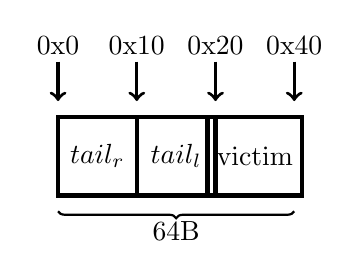
\begin{tikzpicture}
    [%%%%%%%%%%%%%%%%%%%%%%%%%%%%%%
        box/.style={rectangle,draw=black, ultra thick, minimum size=1cm},
    ]%%%%%%%%%%%%%%%%%%%%%%%%%%%%%%

\foreach \y [count=\x] in {$tail_r$, $tail_l$, victim}
{\node[box] at (\x-1,0){\y};}
\draw[decorate,decoration={brace,mirror},thick] (-.5,-.7) -- node[below]{64B} (2.5,-.7);
\draw[->,very thick] (-0.5, 1.2) --  node[above,yshift=2mm]{0x0} (-0.5, .7);
\draw[->,very thick] (0.5,1.2) --  node[above,yshift=2mm]{0x10} (0.5,.7);
\draw[->,very thick] (1.5,1.2) --  node[above,yshift=2mm]{0x20} (1.5,.7);
\draw[->,very thick] (2.5,1.2) --  node[above,yshift=2mm]{0x40} (2.5,.7);
\end{tikzpicture}

\end{document}